\chapter{Network e Port Scanning}
Dal punto di vista dell'\textbf{amministratore} di rete, la scansione è 
un'\textbf{attività preliminare fondamentale} per conoscere quali dispositivi siano 
collegati e configurazione abbiano; l'amministratore può conoscere come sia composto 
il sistema informatico da difendere.

\noindent Dal punto di vista dell'\textbf{attaccante}, accedere a queste informazioni 
permette di sapere a quali \textbf{vulnerabilità} sia esposta la rete (sistemi operativi 
in uso, sw non aggiornato, porte aperte sfruttabili, \dots).

\begin{figure}[H]
    \centering
    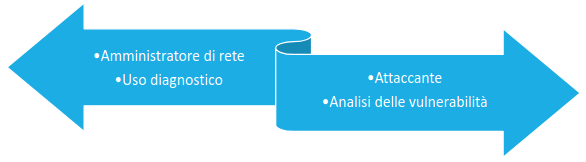
\includegraphics[width=0.9\linewidth]{chapters/9/images/intro.png}
\end{figure}

Le \textbf{attività principali} portate avanti dall'attaccante sono:
\begin{itemize}
    \item la \textbf{mappatura della rete} (network scanning, vedo quali macchine sono attive sulla rete)
    \item riconoscere i servizi UDP e TCP \textbf{disponibili} (port scanning)
    \item riconoscere i \textit{sistemi di filtraggio} usati per l'utente 
    \item determinare i \textit{sistemi operativi} usati 
\end{itemize}

\noindent Sia \textit{network scanning} che \textit{port scanning} sono rilevabili e sono \textbf{illegali}
(salvo autorizzazione del proprietario della rete/macchina).

\noindent Generalmente, salvo alcuni servizi che devono essere esposti verso 
l'esterno (come HTTP/HTTPS nel caso di un server web), il firewall blocca 
questo tipo di richieste.

\section{Tipologie di scansione}
Le scansioni vengono classificate in base al modo in cui sono compiute, al loro scopo e 
al numero di host coinvolti.

\subsection{Numero di host coinvolti}
\begin{itemize}
    \item un singolo host interroga diverse macchine 
    \item tanti host fanno scanning di una sola macchina (si cerca di lasciare meno tracce)
    \item tante macchine fanno scanning di tanti host 
\end{itemize}

\begin{figure}[H]
    \centering
    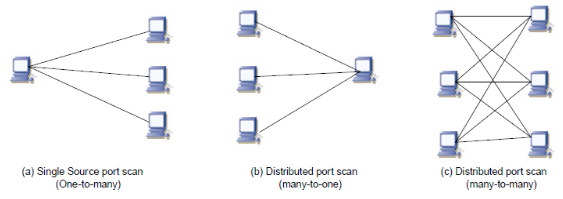
\includegraphics[width=0.9\linewidth]{chapters/9/images/tipi-scansioni.png}
\end{figure}

\subsection{Natura della scansione}
È possibile parlare di scanning:
\begin{itemize}
    \item \textbf{verticale:} più porte di una singola macchina vengono scansionate 
    \item \textbf{Orizzontale:} la stessa porta di più macchine viene controllata 
    \item \textbf{Ibrido:} combinazione delle precedenti
\end{itemize}


\noindent Per quanto riguarda la \textbf{natura della scansione}, 
si può classificare in:
\begin{itemize}
    \item \textbf{Scanning attivo:} si mandano pacchetti alla macchina da scansionare, che 
    possono essere generici o relativi a un particolare protocollo o sw 
    \item \textbf{Scanning passivo:} ci si limita a fare sniffing sulla rete e dedurre come sia 
    configurata la macchina
\end{itemize}

\begin{figure}[H]
    \centering
    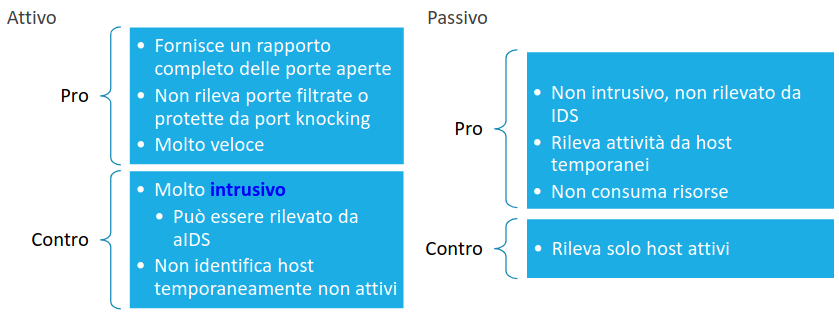
\includegraphics[width=1\linewidth]{chapters/9/images/attivo-passivo.png}
\end{figure}

\subsection{Scopo}
\begin{itemize}
    \item Si parla di \textbf{\textit{wide range scanning}} quando si analizza un 
    dato insieme di indirizzi 
    \item Si parla di \textbf{\textit{target-specific scanning}} quando la scansione 
    riguarda un'entità specifica
\end{itemize}

\section{Risultati (port scanning)}
I risultati di uno scan su una porta possono portare alle seguenti considerazioni:
\begin{itemize}
    \item \textbf{Aperta:} il target ha risposto, indicando che un servizio è in ascolto 
    su quella porta (\textit{connection accepted})
    \item \textbf{Chiusa:} il target ha risposto rifiutando la connessione (\textit{connection denied})
    \item \textbf{Bloccata/Filtrata:} un sistema di sicurezza perimetrale (come un firewall) ha 
    bloccato l'accesso alla porta, impedendo di individuare uno stato (\textit{connection dropped/filtered})
\end{itemize}

\section{Attacchi tramite protocolli noti}
\begin{itemize}
    \item \textbf{ARP scan:} tramite il protocollo ARP è possibile scoprire tutti i dispostivi 
    attivi su una rete locale; l'attacco consiste nel mandare una serie di richieste ARP in broadcast al fine 
    di collezionare tutti gli IP 
    \item \textbf{ICMP:} vengono mandati una serie di pacchetti ICMP \textit{echo request} (ping) per 
    poi rimanere in attesa della risposta (ICMP \textit{echo reply}); spesso questo approccio non è percorribile 
    in quanto i ping vengono spesso bloccati dagli amministratori di rete.

    \noindent Per aggirare questa contromisura, è possibile usare ICMP \textit{timestamp}
    \newpage
    \item \textbf{TCP:} sono possibili due approcci che sfruttano questo protocollo:
    \begin{itemize}
        \item \textbf{TCP SYN ping:} si manda un TCP SYN; nel caso in cui si riceve risposta SYN-ACK, 
        il servizio è attivo su quella porta 
        \item \textbf{TCP ACK ping:} si manda un pacchetto ACK; nel caso in cui si riceve risposta 
        RST, il servizio è attivo su quella porta 
    \end{itemize}
    \item \textbf{UDP ping:} si manda un pacchetto UDP vuoto; se l'host risponde, sappiamo che è attivo 
    su quella porta 
    \item \textbf{IP ping:} si mandano pacchetti con protocolli non abilitati (nell'header IP è prevista l'indicazione del protocollo) e 
    si verifica se l'host risponde (analogo a UDP ping)
\end{itemize}

\subsection{TCP connect scan}
È un attacco che fa uso della \textit{syscall} \texttt{connect()} per connettersi ad una 
socket esposta sulla rete in stato di listen.

\subsubsection{Open scan}
Le risposte ad un SYN possono essere:
\begin{itemize}
    \item SYN-ACK: porta aperta 
    \item RST: porta chiusa 
    \item \textit{nessuna rispsota} : porta filtrata da firewall
    \item ICMP unreachable: porta filtrata da un firewall
\end{itemize}

\subsubsection{Half-open scan}
Nel caso in cui si riceva un SYN-ACK, si restituisce un RST per \textbf{terminare la connessione}
TCP rimasta aperta.

\noindent Questo approccio è meno intruviso e quindi meno rilevabile.

\subsection{Stealth scan}
Gli attacchi di \textit{stealth scan} possono essere fatti in vari modi:
\begin{itemize}
    \item \textbf{SYN-ACK scan:} le richieste SYN sono spesso individuate e filtrate; si può invece 
    mandare un pacchetto SYN-ACK e dedurre informazioni dalla risposta
    \begin{itemize}
        \item se la risposta è RST, la porta è chiusa 
        \item se non si riceve risposta, la porta è aperta (si possono avere falsi positivi, ad 
        esempio per \textit{packet loss})
    \end{itemize}
    \item \textbf{ACK scan:} prevede di mandare un pacchetto ACK direttamente (non si mira a vedere 
    se una porta è aperta):
    \begin{itemize}
        \item se la risposta è RST, la porta \textit{non è filtrata}
        \item se non si riceve risposta o \textit{ICMP unreachable}, la porta \textit{è filtrata}
    \end{itemize}

    \noindent $\rightarrow$ questo attacco mira ad \textbf{individuare la presenza di un firewall}
    \item \textbf{Window scan:} è simile ad un ACK scan, si basa siò \textit{window size} presente nel 
    pacchetto TCP 
    \begin{itemize}
        \item RST e $window \neq 0 \rightarrow$ porta aperta 
        \item RST e $window = 0 \rightarrow$ porta chiusa 
        \item nessuna riposta o \textit{ICMP unreachable} $\rightarrow$ porta filtrata
    \end{itemize}
    \item \textbf{FIN, XMAS, NULL scan:} in questo attacco si punta ad impostare a 0/1 alcuni flag 
    dell'header TCP; nello specifico:
    \begin{itemize}
        \item FIN
        \item URG 
        \item PSH
    \end{itemize}

    \noindent Gli attacchi operano in questo modo:
    \begin{itemize}
        \item \textbf{FIN:} mette a 1 solo il flag FIN 
        \item \textbf{NULL:} mette a 0 tutti i flag 
        \item \textbf{XMAS:} \textit{spegne} e \textit{accende} in maniera casuale tutti i flag (come 
        le luci di natale)
    \end{itemize}

    \noindent In base alla rispota, si può capire se la porta è aperta, chiusa oppure filtrata. Questo attacco 
    permette di scavalcare alcuni firewall ceh filtrano solo SYN e ACK.
    \item \textbf{TCP fragmentation scan:} invia dei frammenti di pacchetti; aumenta la difficoltà di detection ma 
    è lento, non affidabile e potrebbe mandare in crush il firewall (si viene individuati)
    \item \textbf{Idle scan:} non si inviano i pacchetti direttamente alla vittima, ma si utilizza 
    un intermediario; in questo modo si riesce a non apparire nella connessione con il server
    \item \textbf{FTP bounce scan:} simile all'\textit{idle scan} (server FTP agisce da zombie), usa il protocollo FTP (File Transfer Protocol);
    se il server FTP è in modalità attiva, con il comando PORT si può indicare su quale IP e porta 
    ricevere la risposta (si usano quelli della vittima).

    \noindent Se il server non riesce a collegarsi, darà un errore sulla connessione FTP all'attaccante.

    \noindent Ha il vantaggio di essere \textit{stealth}, ma funziona solo con TCP, è lento e 
    lascia tracce sul server FTP
\end{itemize}

\section{OS fingerprint}
È un attacco in cui l'obiettivo è \textbf{identificare il sistema operativo} usato dalla vittima.
Si guardano le eventuali risposte e da esse si cerca di capire qual è il sistema operativo (ci 
sono delle picolle differenze).

\noindent Ci si può difendere usando dei firewall o cambiando la firma del TCP/IP stack, usando
quella di un altro sistema operativo per ingannare l'attaccante.



































